\documentclass[10pt]{scrartcl}

\usepackage[utf8]{inputenc}
\usepackage{tabularx}
\usepackage[ngerman]{babel}
\usepackage[automark]{scrpage2}
\usepackage{amsmath,amssymb,amstext}
%\usepackage{mathtools}
\usepackage[]{color}
\usepackage[]{enumerate}
\usepackage{graphicx}
\usepackage{lastpage}
\usepackage[perpage,para,symbol*]{footmisc}
\usepackage{listings} 
\usepackage[pdfborder={0 0 0},colorlinks=false]{hyperref}
\usepackage[numbers,square]{natbib}
\usepackage{color}
\usepackage{colortbl}
\usepackage{listings}
\usepackage{a4wide}
\usepackage{xspace}
\usepackage{listings}
\usepackage{hyperref}
\usepackage{epstopdf}

\lstset{numbers=left, numberstyle=\tiny, numbersep=5pt, breaklines=true, showstringspaces=false} 

%changehere
\def\titletext{TH1 Praktikum 2 : Ausarbeitung}
\def\titletextshort{Praktikum 2}
\author{Carsten Noetzel, Armin Steudte}

\title{\titletext}

%changehere Datum der Übung
\date{23.03.2012}

\pagestyle{scrheadings}
%changehere
\ihead{TH1, Padberg}
\ifoot{Generiert am:\\ \today}

\cfoot{Carsten Noetzel, Armin Steudte}


\ohead[]{\titletextshort}
\ofoot[]{{\thepage} / \pageref{LastPage}}

\setlength{\parindent}{0.0in}
\setlength{\parskip}{0.1in}

\begin{document}
\maketitle

\setcounter{tocdepth}{3}
\tableofcontents
\listoffigures
%\lstlistoflistings

\section{Aufgabe 1}
In dieser Aufgabe ist eine Modelleisenbahn in Form eines Kreises zu modellieren.
Dabei sollen folgende Aspekte beachtet werden:
\begin{itemize}
	\item Es sollen mindestens 8 Gleisabschnitte geben.
	\item Zügen sollen sowohl vorwärts als auch rückwärts fahren können.
	\item Es dürfen sich nicht zwei Züge gleichzeitig auf einem Gleisabschnitt befinden.
	\item Es soll zwei Züge geben.
\end{itemize}
Im Folgenden sollen diese Aspekte in der oben genannten Reihenfolge betrachtet werden.

\subsection{Streckenmodellierung}
Ein Gleisabschnitt wird im Modell in Form einer Stelle mit der Kapazität von eins modelliert.
Gleichzeitig existiert pro Gleisabschnitt eine zusätzliche Stelle mit einer Kapazität von eins, welche den Zustand eines Gleisabschnitts angibt.
Sie wird initial mit einem Token belegt, was bedeutet dass dieser Gleisabschnitt nicht von einem Zug befahren wird und damit befahren werden kann.
Kein Token auf der Stelle signalisiert einen nicht befahrbaren Gleisabschnitt.\\
Züge werden durch Token auf den Stellen dargestellt, die sich auf den Gleisabschnitts-Stellen bewegen.
Ihre Bewegung wird dabei über das Schalten von Transitionen realisiert.
Für jede Bewegungsrichtung existiert eine Transition $t_{1}$ zwischen zwei Stellen $p_{1}$ und $p_{2}$.
Für das Vorwärtsfahren bzw. die Hinrichtung existiert zwei Kanten $(p_{1},t_{1})$ und $(t_{1},p_{2})$. Diese verbinden $p_{1}$ mit $t$ und $t_{1}$ zusätzlich mit $p_{2}$.
Das Rückwärtsfahren bzw. die Rückrichtung wird durch eine weite Transition $t_{2}$ und den dazugehörigen Kanten $(p_{2},t_{2})$ sowie $(t_{2},p_{1})$ simuliert.

\subsection{Exklusives Befahren eines Gleisabschnitts}
Wechselt ein Zug in den nächsten Gleisabschnitt so wird der Stelle, welche den Zustand zum Befahren eines Gleisabschnitts angibt, das Token entzogen.
Diese Stellen agieren als Vorbedingung für die Transitionen die den Zug auf den ihnen zugeordneten Gleisabschnitt fahren lässt.
Ist kein Token auf der Stelle, und damit der Strecken abschnitt nicht befahrbar, kann sowohl die Transition die den Zug im Uhrzeigersinn als auch die Transition die den Zug gegen den Uhrzeigersinn fahren lässt, nicht schalten.\\
Schaltet ein Transition so wird das Token an die Stelle davor zurückgegeben.
Auf diese Weise kann nur ein Zug zur selben Zeit einen Gleisabschnitt befahren.

\subsection{Zugmodellierung}
Züge werden durch Token auf Gleisabschnitts-Stellen modelliert.
Zwei Züge sind damit zwei Token die sich auf unterschiedlichen Stellen befinden.

\section{Aufgabe 3}

\subsection{S-Invarianten}
Mit Hilf des Tools Netlab wurde den die folgenden S-Invarianten berechnet.

\begin{figure}[htbp]
	\centering	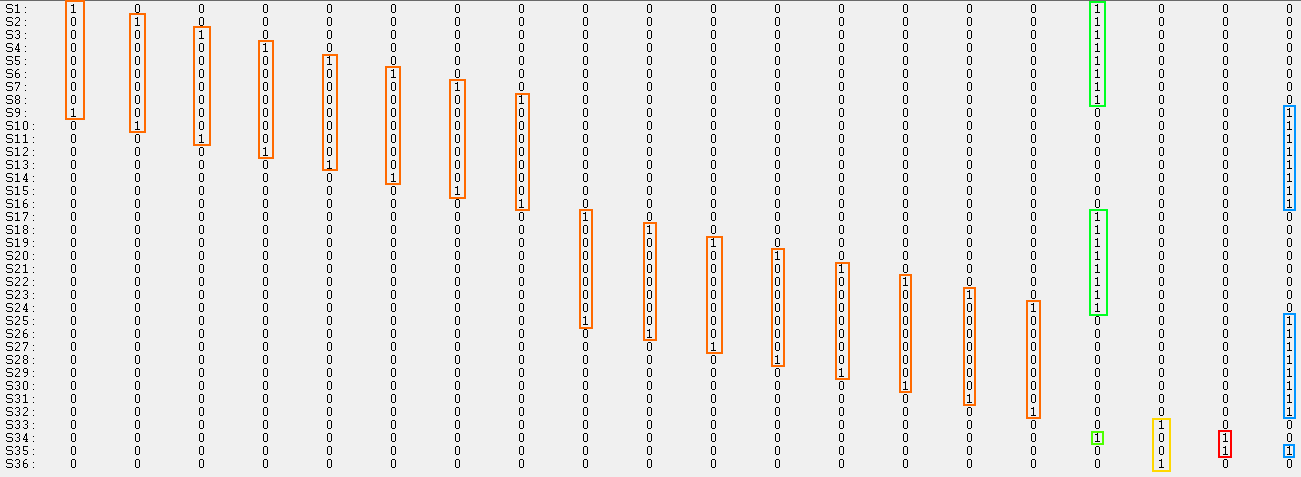
\includegraphics[width=1.0\textwidth]{Bilder/s_invarianten.png}
	\caption{S-Invarianten des Netzes aus Aufgabe 2}
	\label{fig:s_invarianten}
\end{figure}

Die orange markierten Invarianten repräsentieren die Beziehung zwischen Gleisabschnitt (z.B. S1) und Token (z.B. S)), welches einen freien Gleisabschnitt signalisiert.
Diese Invarianten sagen aus, dass jeweils immer nur ein Zug einen Gleisabschnitt befahren kann.\\

Die grün markierten Invarianten beschreibt die Zusammenhänge der Stellen-Kreise (S1-S9; S17-S24) auf denen die Züge fahren.
Dass alle Stellen in den Kreisen eine Gewicht von 1 besitzen, ist sichergestellt das beim Bewegen des Zuges keine neuen Züge erstellt werden.
Es werden nur existierende Züge fortbewegt.
Die Stelle S34 in dieser Invariante symbolisiert die Weiche, auch bei ihr ist sichergestellt dass keine neuen Züge erstellt werden.\\
  
Die blauen Markierungen repräsentieren den gleichen Aspekt für Stellen welche die "`Freitokens"' beinhalten und zur Signalisierung eines freien Gleisabschnitts dienen.
Eine Gewichtung von 1 sagt dabei in diesem Fall aus, dass keine neuen "`Freitokens"' erzeugt werden und somit sichergestellt ist, dass sich immer nur ein Zug auf einem Gleisabschnitt befinden kann.\\

Das Schaltverhalten der eingebauten Schranke wird durch die gelb markierte Invariante beschrieben.
Sie beschreibt, dass die Schranke nie gleichzeitig offen und geschlossen sein kann, was in der Aufgabenstellung auch gefordert wurde.\\

Durch die rote Invariante ist sichergestellt, dass die Weiche nur durch einen Zug befahren werden kann und es ist sichergestellt dass beim Befahren der Weiche keine neuen Züge erzeugt werden.

\subsection{T-Invarianten}
Für das Netz aus Aufgabe 2 wurden von Netlab die folgenden T-Invarianten berechnet.

\begin{figure}[htbp]
	\centering	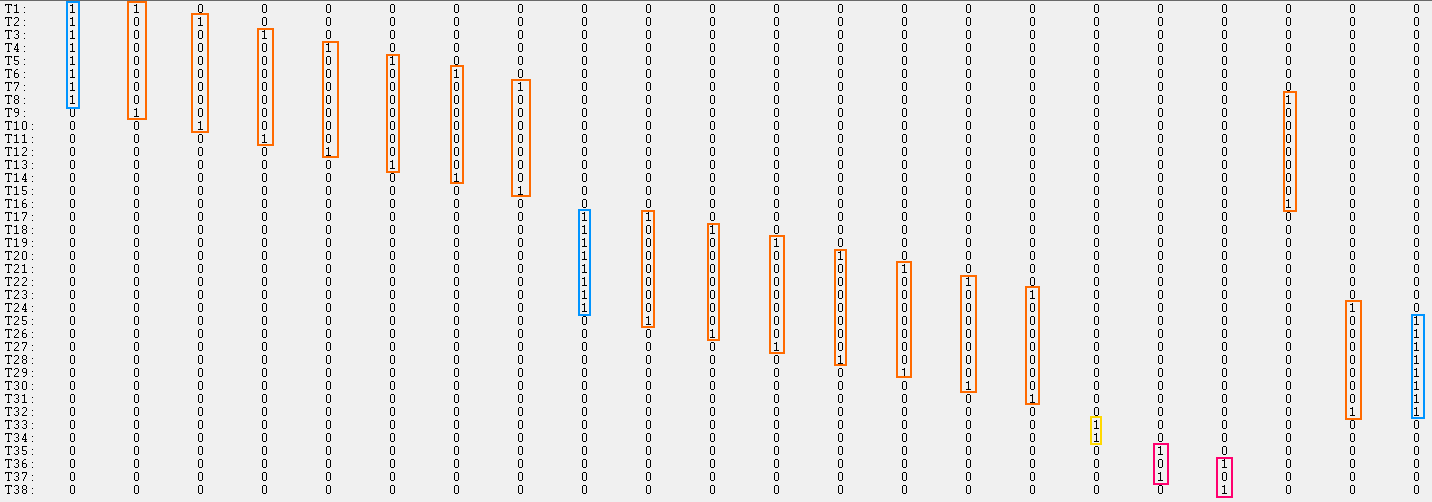
\includegraphics[width=1.0\textwidth]{Bilder/t_invarianten.png}
	\caption{T-Invarianten des Netzes aus Aufgabe 2}
	\label{fig:T_invarianten}
\end{figure}

Die Zyklen innerhalb des Petrinetzes, die das Befahren der beiden Kreise in Vorwärts- und Rückwärtsrichtung darstellen, wurden in den T-Invarianten blau markiert.
Da Netlab nur einen Teil der T-Invarianten hier anzeigt, fehlt hier leider das Befahren des linken Kreises in Vorwärtsrichtung.
Generell zeigen aber die Invarianten, dass beide kreisförmigen Gleisabschnitt sowohl vorwärts als auch rückwärts durchgängig befahren werden können.\\

Die orangen Markierungen bedeuten, dass alle Gleisabschnitte sowohl vorwärts als auch rückwärts befahren werden können.
Auch hier wird durch Netlab nur ein Teil der dazugehörigen Invarianten berechnet.
Ein Beispiel sind die Transitionen T1 und T9 die zusammen mit der Stelle 1 das Vorwärts- sowie Rückwärtsfahren des ersten Gleisabschnitts realisieren.\\

Die Weiche wird in den T-Invarianten durch die roten Markierungen sichtbar.
Der Zyklus hierbei beschreibt, dass in unserer Modellierung es möglich ist Züge auf den Gleisabschnitt der Weiche rauf- und runterfahren zu lassen.
Dieses ist von beiden Kreisen aus möglich.
Diese Eigenschaft war nicht explizit gefordert, widerspricht aber auch nicht der Aufgabenstellung.\\

Das Schalten der Schranke zwischen dem geöffneten und geschlossenem Zustand kann an der Gelben Markierung festgemacht werden.
Es ist somit sichergestellt, dass sich die Schranke nur in einem dieser beiden Zustände befindet und es keine nicht definierten Zustände gibt. 
 

\section{Aufgabe 2}
In dieser Aufgabe ist eine Modelleisenbahn in Form einer acht zu modellieren.
Dabei sollen folgende Aspekte beachtet werden:
\begin{itemize}
	\item Es sollen eine Schranke geben.
	\item Züge dürfen die Schranke nur passieren, wenn die die Schranke geschlossen ist.
	\item Es soll eine Weiche geben, die die beiden Kreise zu einer acht verbindet.
	\item Die Weiche soll in beide Richtungen befahrbar sein.
\end{itemize}
Im Folgenden sollen diese Aspekte in der oben genannten Reihenfolge betrachtet werden.

\subsection{Umsetzung der Schranke}
Abbildung \ref{fig:Schranke} zeigt die im Schienennetz eingebrachte Schranke zwischen dem ersten und dritten Gleisabschnitt. Ein Zug der auf Gleisabschnitt 1 steht und mittels der Transition "`rückwärts"' Gleisabschnitt 2 befahren will, hat als Vorbedingung die Stelle "`Schranke geschlossen"' und "`Abschnitt 2 frei"'. Damit wird sichergestellt, dass Gleisabschnitt 2 immer nur dann befahren werden kann, wenn die Schranke geschlossen und der Abschnitt nicht von einem Zug belegt ist. Gleiches gilt für Gleisabschnitt 3 bei Zügen die mittels der Transition "`vorwärts"' auf Gleisabschnitt 2 vorrücken wollen.\\
Die Schranke kann mittels der Transitionen "`Schranke öffnen"' und "`Schranke schließen"' geöffnet und geschlossen werden.
 
\begin{figure}[htbp]
	\centering	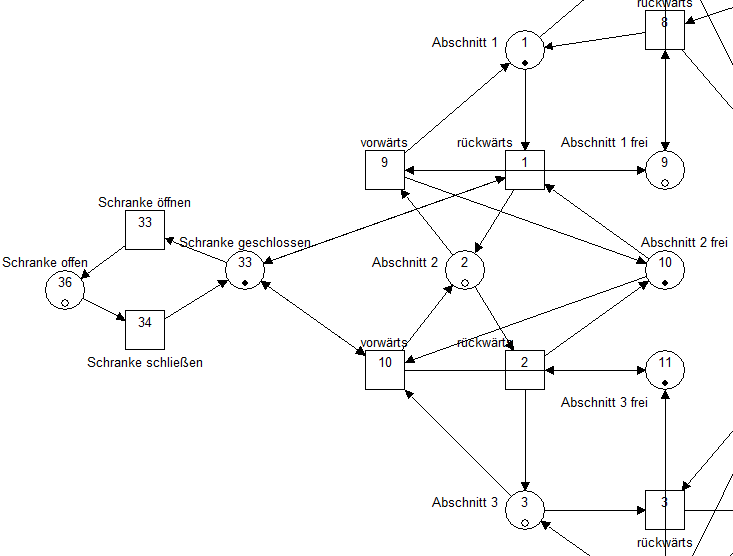
\includegraphics[width=1.0\textwidth]{Bilder/Aufgabe2_Schranke.png}
	\caption{Umsetzung der Schranke}
	\label{fig:Schranke}
\end{figure}

\subsection{Umsetzung der Weiche}
Abbildung \ref{fig:Weiche} zeigt die im Gleisnetz eingebrachte Weiche, die die beiden kreisförmigen Strecken zu einer acht verbindet.\\
Ein Zug der auf Gleisabschnitt 6 steht, kann mittels der Transition "`nehme Abzweigung"' die Abzweigung befahren, um zum rechten kreisförmigen Segment zu gelangen, wenn die Abzweigung frei ist. Nimmt ein Zug auf Gleisabschnitt 6 die Abzweigung so, wird durch die Transition "`nehme Abzweigung"' der entsprechende Gleisabschnitt wieder auf frei gesetzt, das der Zug sich nun auf der Abzweigung befindet. Gleich gilt für Züge die sich auf Gleisabschnitt 2 im rechten kreisförmigen Segment befinden  und zum linken kreisförmigen Segment wechseln wollen.\\
Nutzt ein Zug die Abzweigung, ist die Stelle  "`Abzweigung"' belegt. Die Transition  "`verlasse Abzweigung"' wird aktiviert wenn Gleisabschnitt 2 bzw. Gleisabschnitt 6 frei sind und ermöglichen es dem Zug, der sich auf der Abzweigung befindet wieder in den kreisförmigen Verkehr einzusteigen.\\
Mit dieser Modellierung ist sichergestellt, dass die Abzweigung in beide Richtungen befahren werden und auch in beide Richtungen verlassen werden kann. Zu jedem Zeitpunkt darf sich immer nur ein Zug auf der Abzweigung befinden.

\begin{figure}[htbp]
	\centering	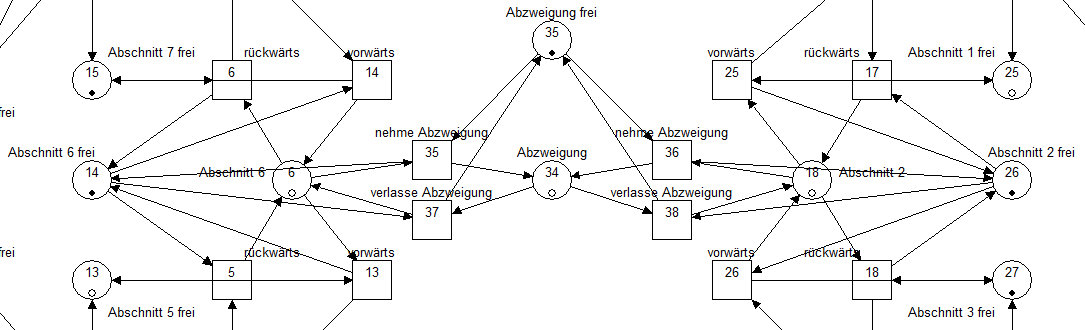
\includegraphics[width=1.0\textwidth]{Bilder/Aufgabe2_Weiche.png}
	\caption{Umsetzung der Weiche}
	\label{fig:Weiche}
\end{figure}

\end{document}

\section{Aufgabe 3}
\subsection{Verhalten mit mehreren Zügen}
Setzt man von Beginn an eine größere Anzahl von Zügen auf das Streckennetz, so haben die Züge weniger Möglichkeiten sich zu bewegen, da mehr Gleisabschnitte blockiert sind. Aus diesem Grund verkleinert sich der Erreichbarkeitsgraph des Netzes mit dem jedem Zug der hinzugefügt wird solange, bis alle Gleisabschnitt besetzt sind und es damit keine Bewegungsmöglichkeiten mehr gibt. Ein solche Situation würde einen Erreichbarkeitsgraphen mit der Anfangsmarkierung erzeugen der keine Kanten besitzt, da keine Transition schalten kann, die einen Zug bewegt. Als Ausnahme hiervon ist das öffnen und schließen der Schranke zu sehen, das unabhängig von den Zügen geschehen kann.

